% Relocalization phase storyboard:
% <1> Previous-phase reference (what is reused)
% <2> Captured point photos (replace paths)
% <3-> Didactic nearest-point graphs (replace paths)

\vspace{-0.3cm}
\begin{columns}[T,onlytextwidth]
  % ---------------- LEFT: VISUAL PANEL ----------------
  \begin{column}{0.63\textwidth}
    \begin{outlinecard}[{\only<1>{Recorded Reference}\only<2-7>{Point Validation (Photo + Graph)}}]
      \centering

      % STEP 1
      \only<1>{
        \begin{tikzpicture}[x=1cm,y=1cm]
          \draw[draw=NavyBlue!45, line width=0.9pt, rounded corners=1.4pt, fill=white]
            (0.10,0.22) rectangle (7.3,3.9);
          \node[inner sep=0pt, anchor=south west] at (0.30,0.44)
            {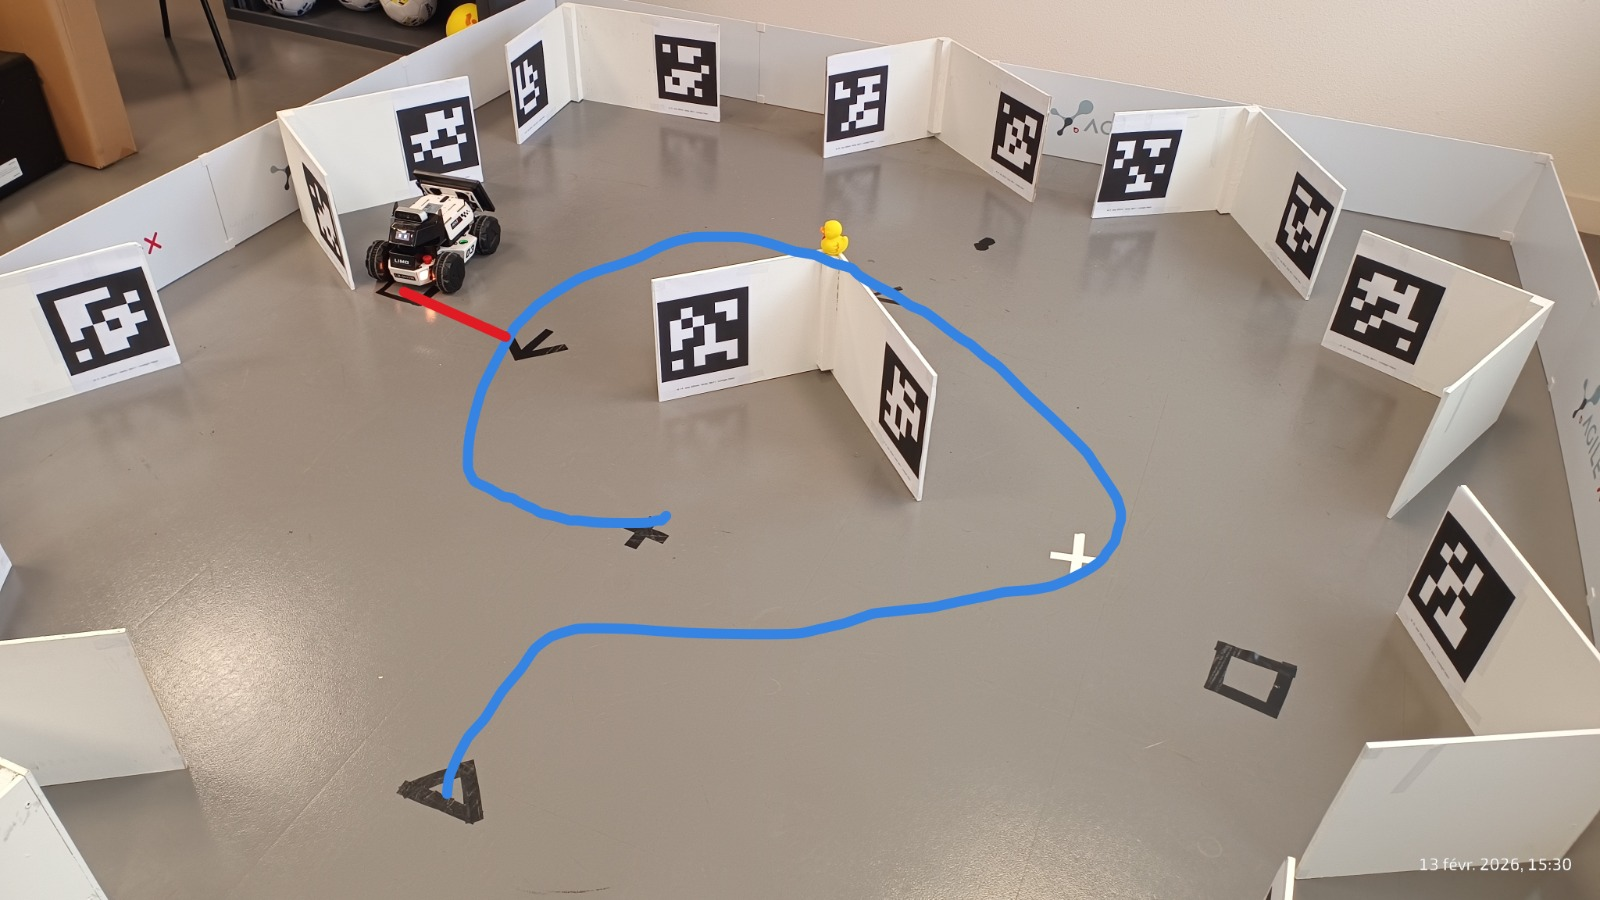
\includegraphics[width=6.7cm,height=3.25cm]{assets/relocphase_1.jpeg}};
          \fill[black, opacity=0.15] (0.30,0.44) rectangle (7.00,3.69);
        \end{tikzpicture}
      }

      % STEP 2
      \only<2-7>{
        \begin{tikzpicture}[x=1cm,y=1cm]
          % Pair 1: 002
          \only<2>{
            \node[anchor=south west, inner sep=0pt] at (0.30,0.34)
              {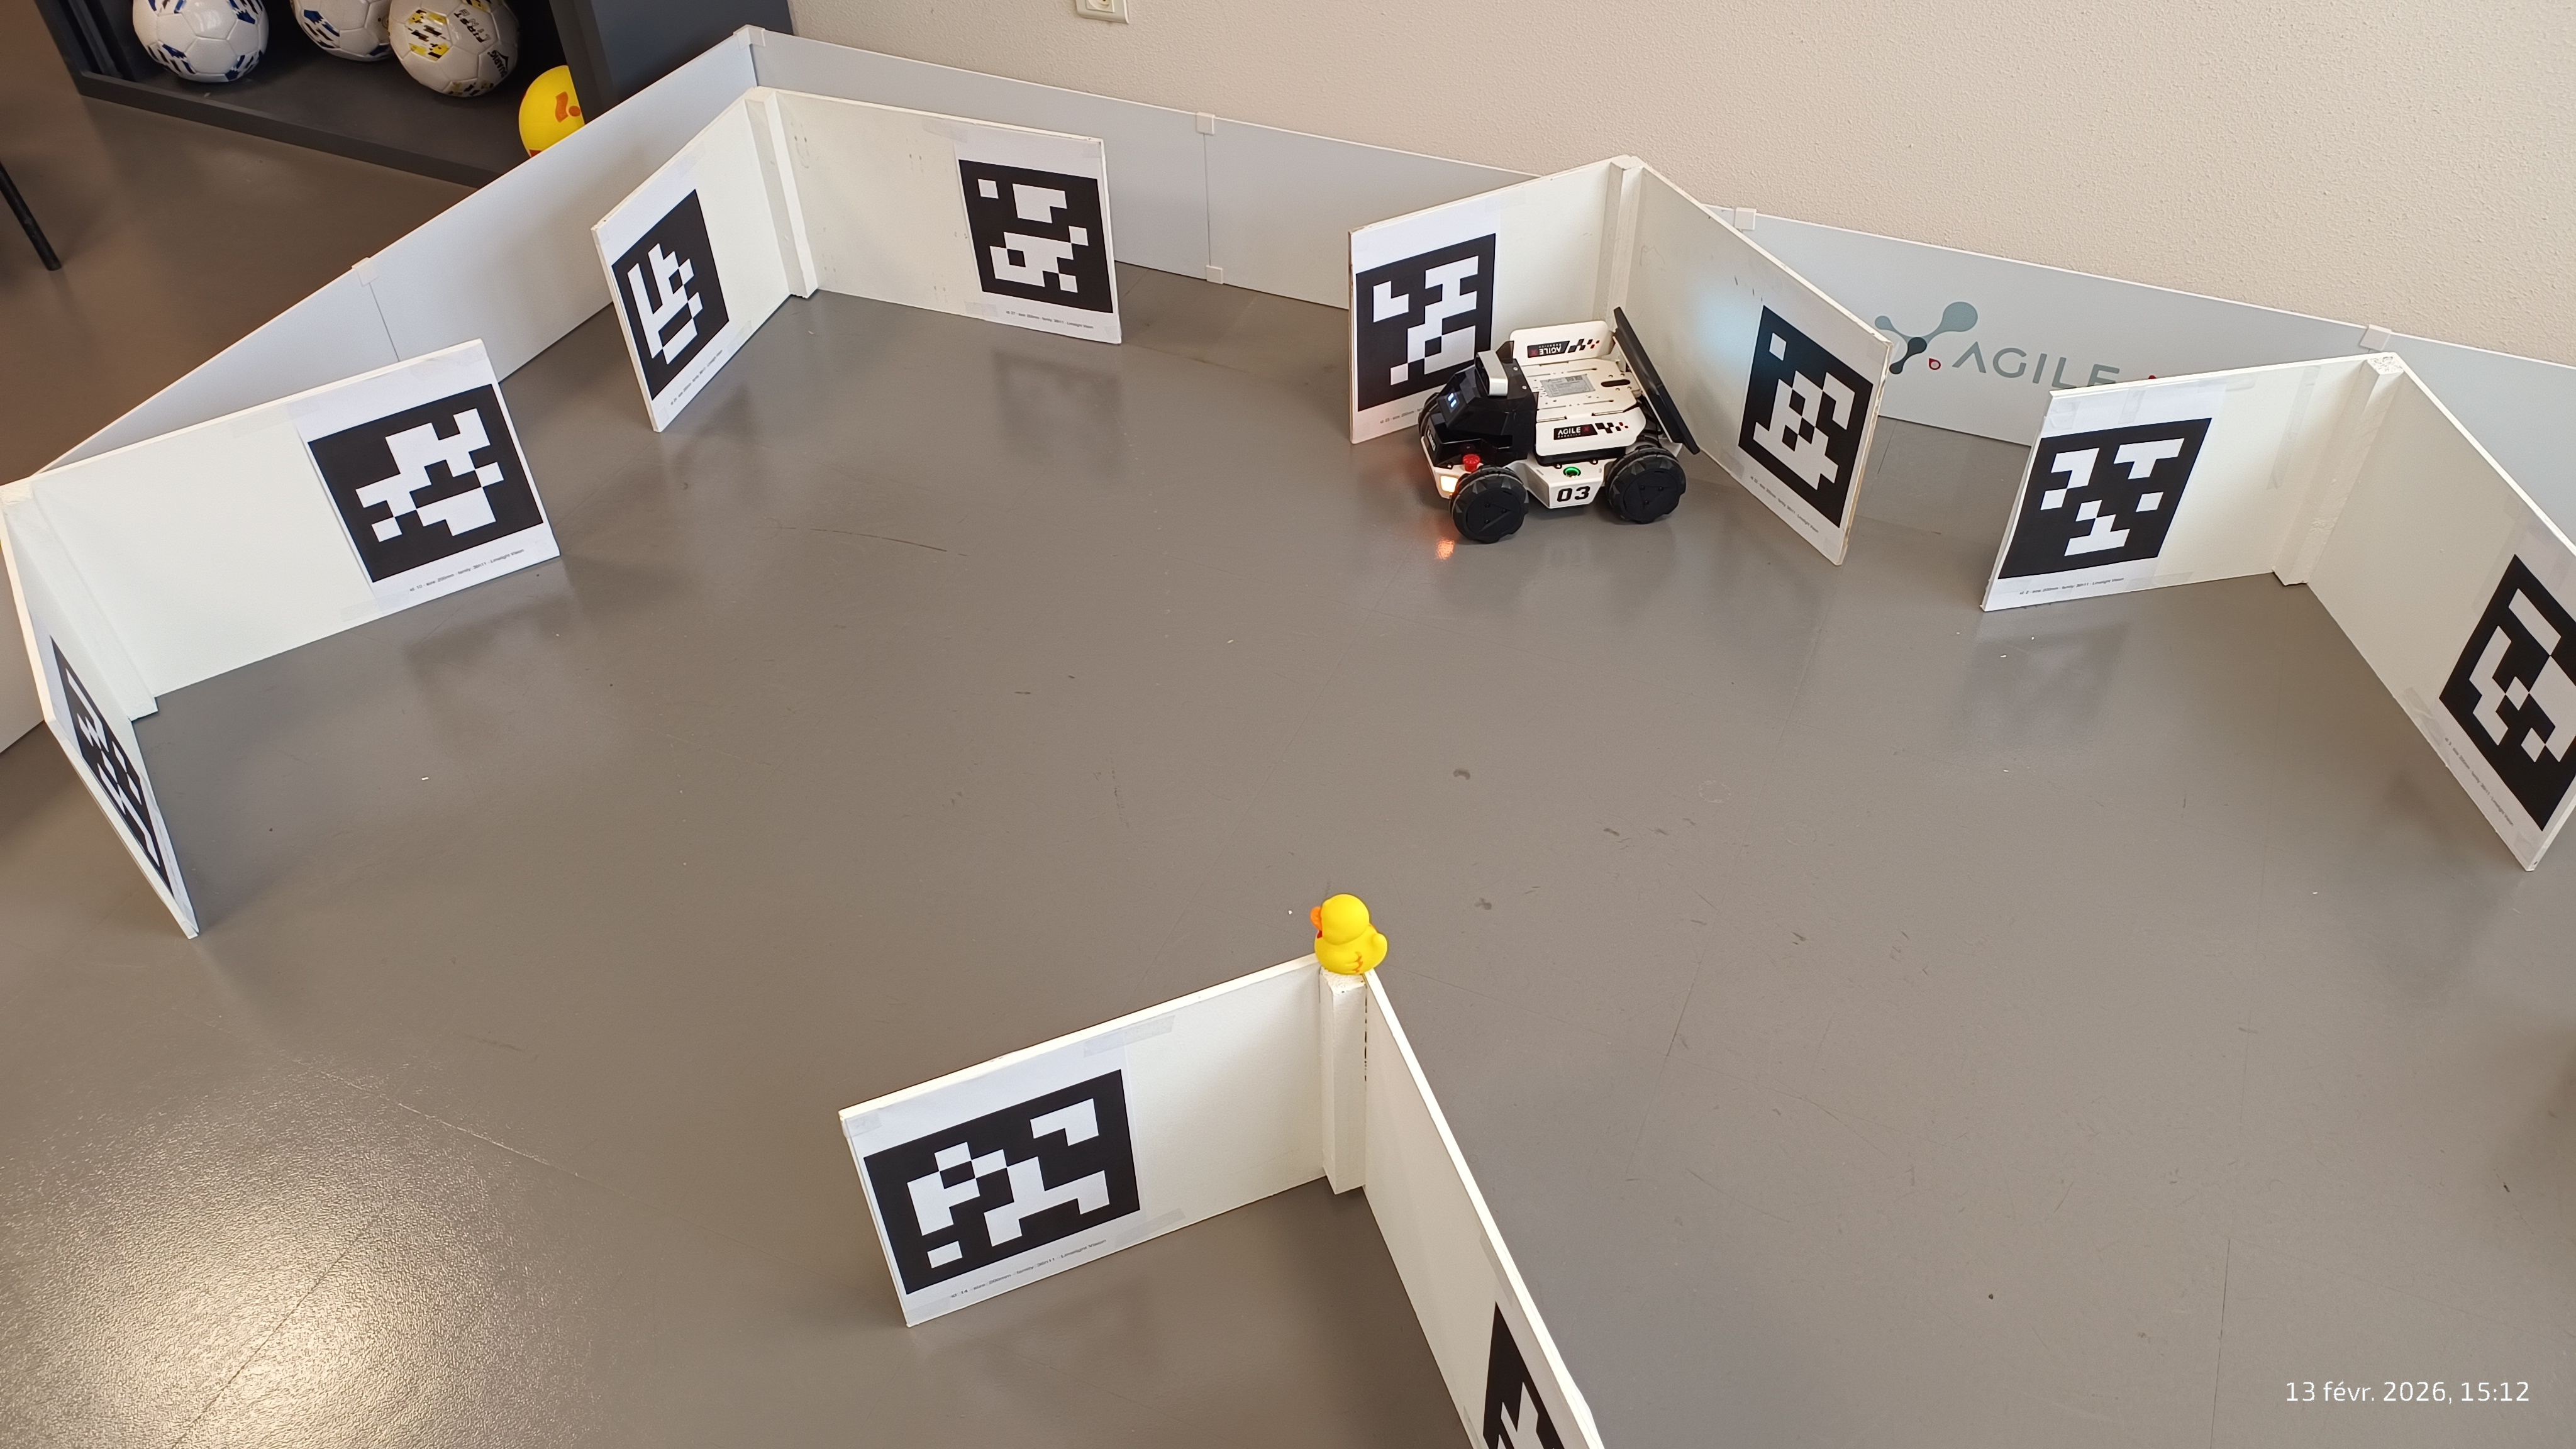
\includegraphics[width=3.35cm,height=3.30cm]{../assets/results/real_s1_reloc_002_foto.jpg}};
            \node[anchor=south west, inner sep=0pt] at (3.85,0.34)
              {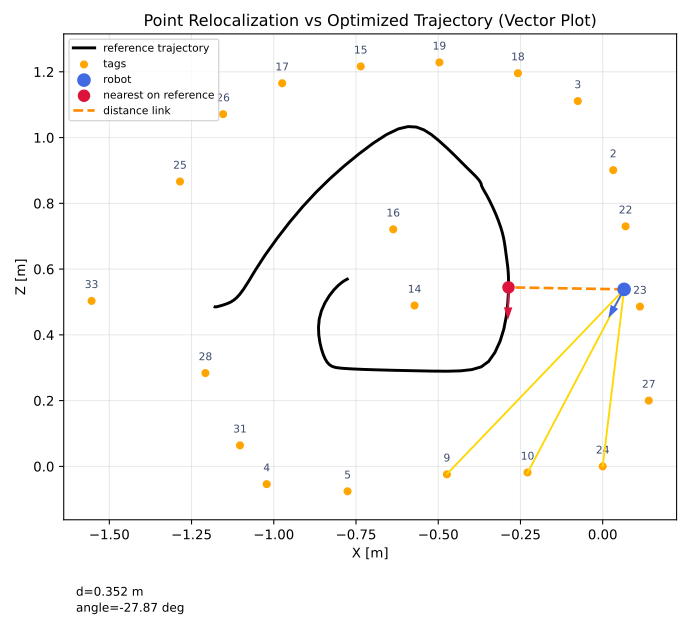
\includegraphics[width=3.35cm,height=3.30cm]{assets/results/graph_002.png}};
            \node[font=\scriptsize\bfseries, text=NavyBlue, anchor=north] at (1.98,0.30) {Point 002};
            \node[font=\scriptsize\bfseries, text=NavyBlue, anchor=north] at (5.53,0.30) {Graph 002};
          }
          % Pair 2: 012
          \only<3>{
            \node[anchor=south west, inner sep=0pt] at (0.30,0.34)
              {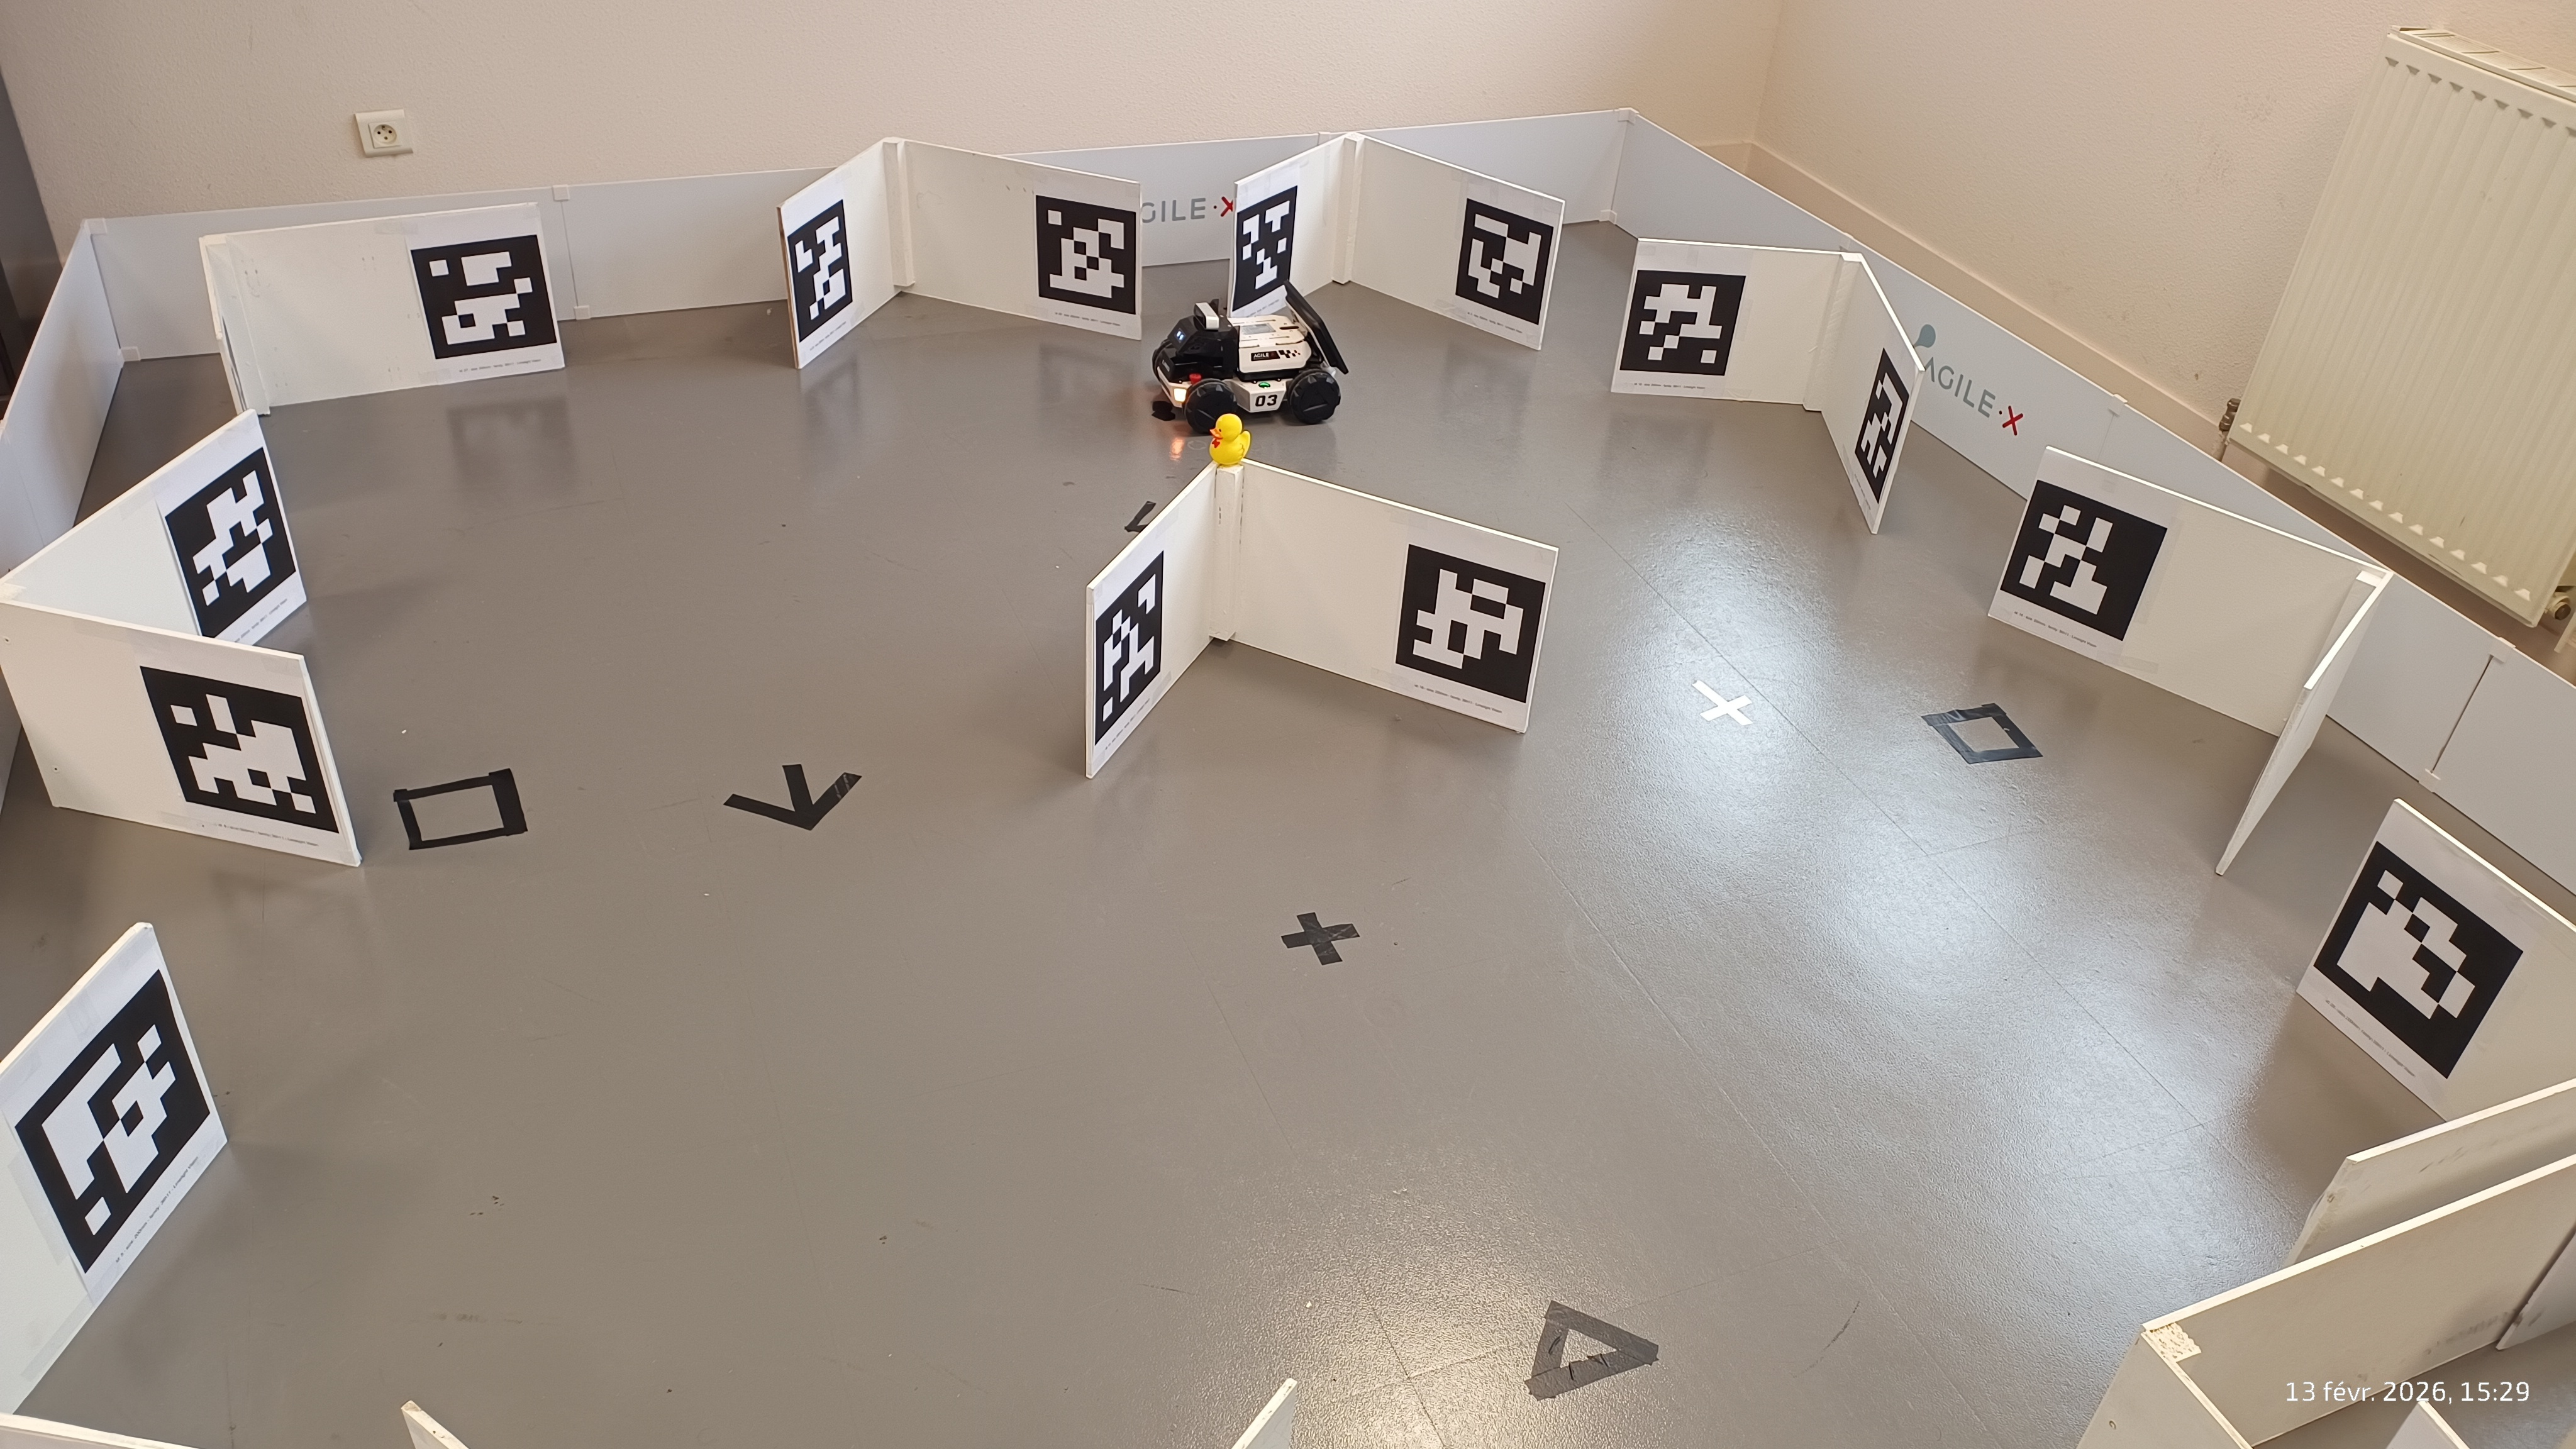
\includegraphics[width=3.35cm,height=3.30cm]{../assets/results/real_s1_reloc_012_foto.jpg}};
            \node[anchor=south west, inner sep=0pt] at (3.85,0.34)
              {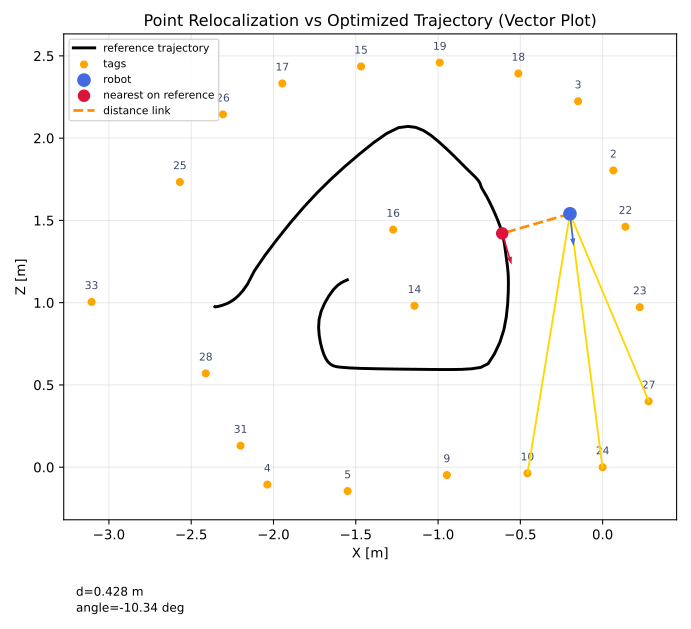
\includegraphics[width=3.35cm,height=3.30cm]{assets/results/graph_012.png}};
            \node[font=\scriptsize\bfseries, text=NavyBlue, anchor=north] at (1.98,0.30) {Point 012};
            \node[font=\scriptsize\bfseries, text=NavyBlue, anchor=north] at (5.53,0.30) {Graph 012};
          }
          % Pair 3: 013
          \only<4>{
            \node[anchor=south west, inner sep=0pt] at (0.30,0.34)
              {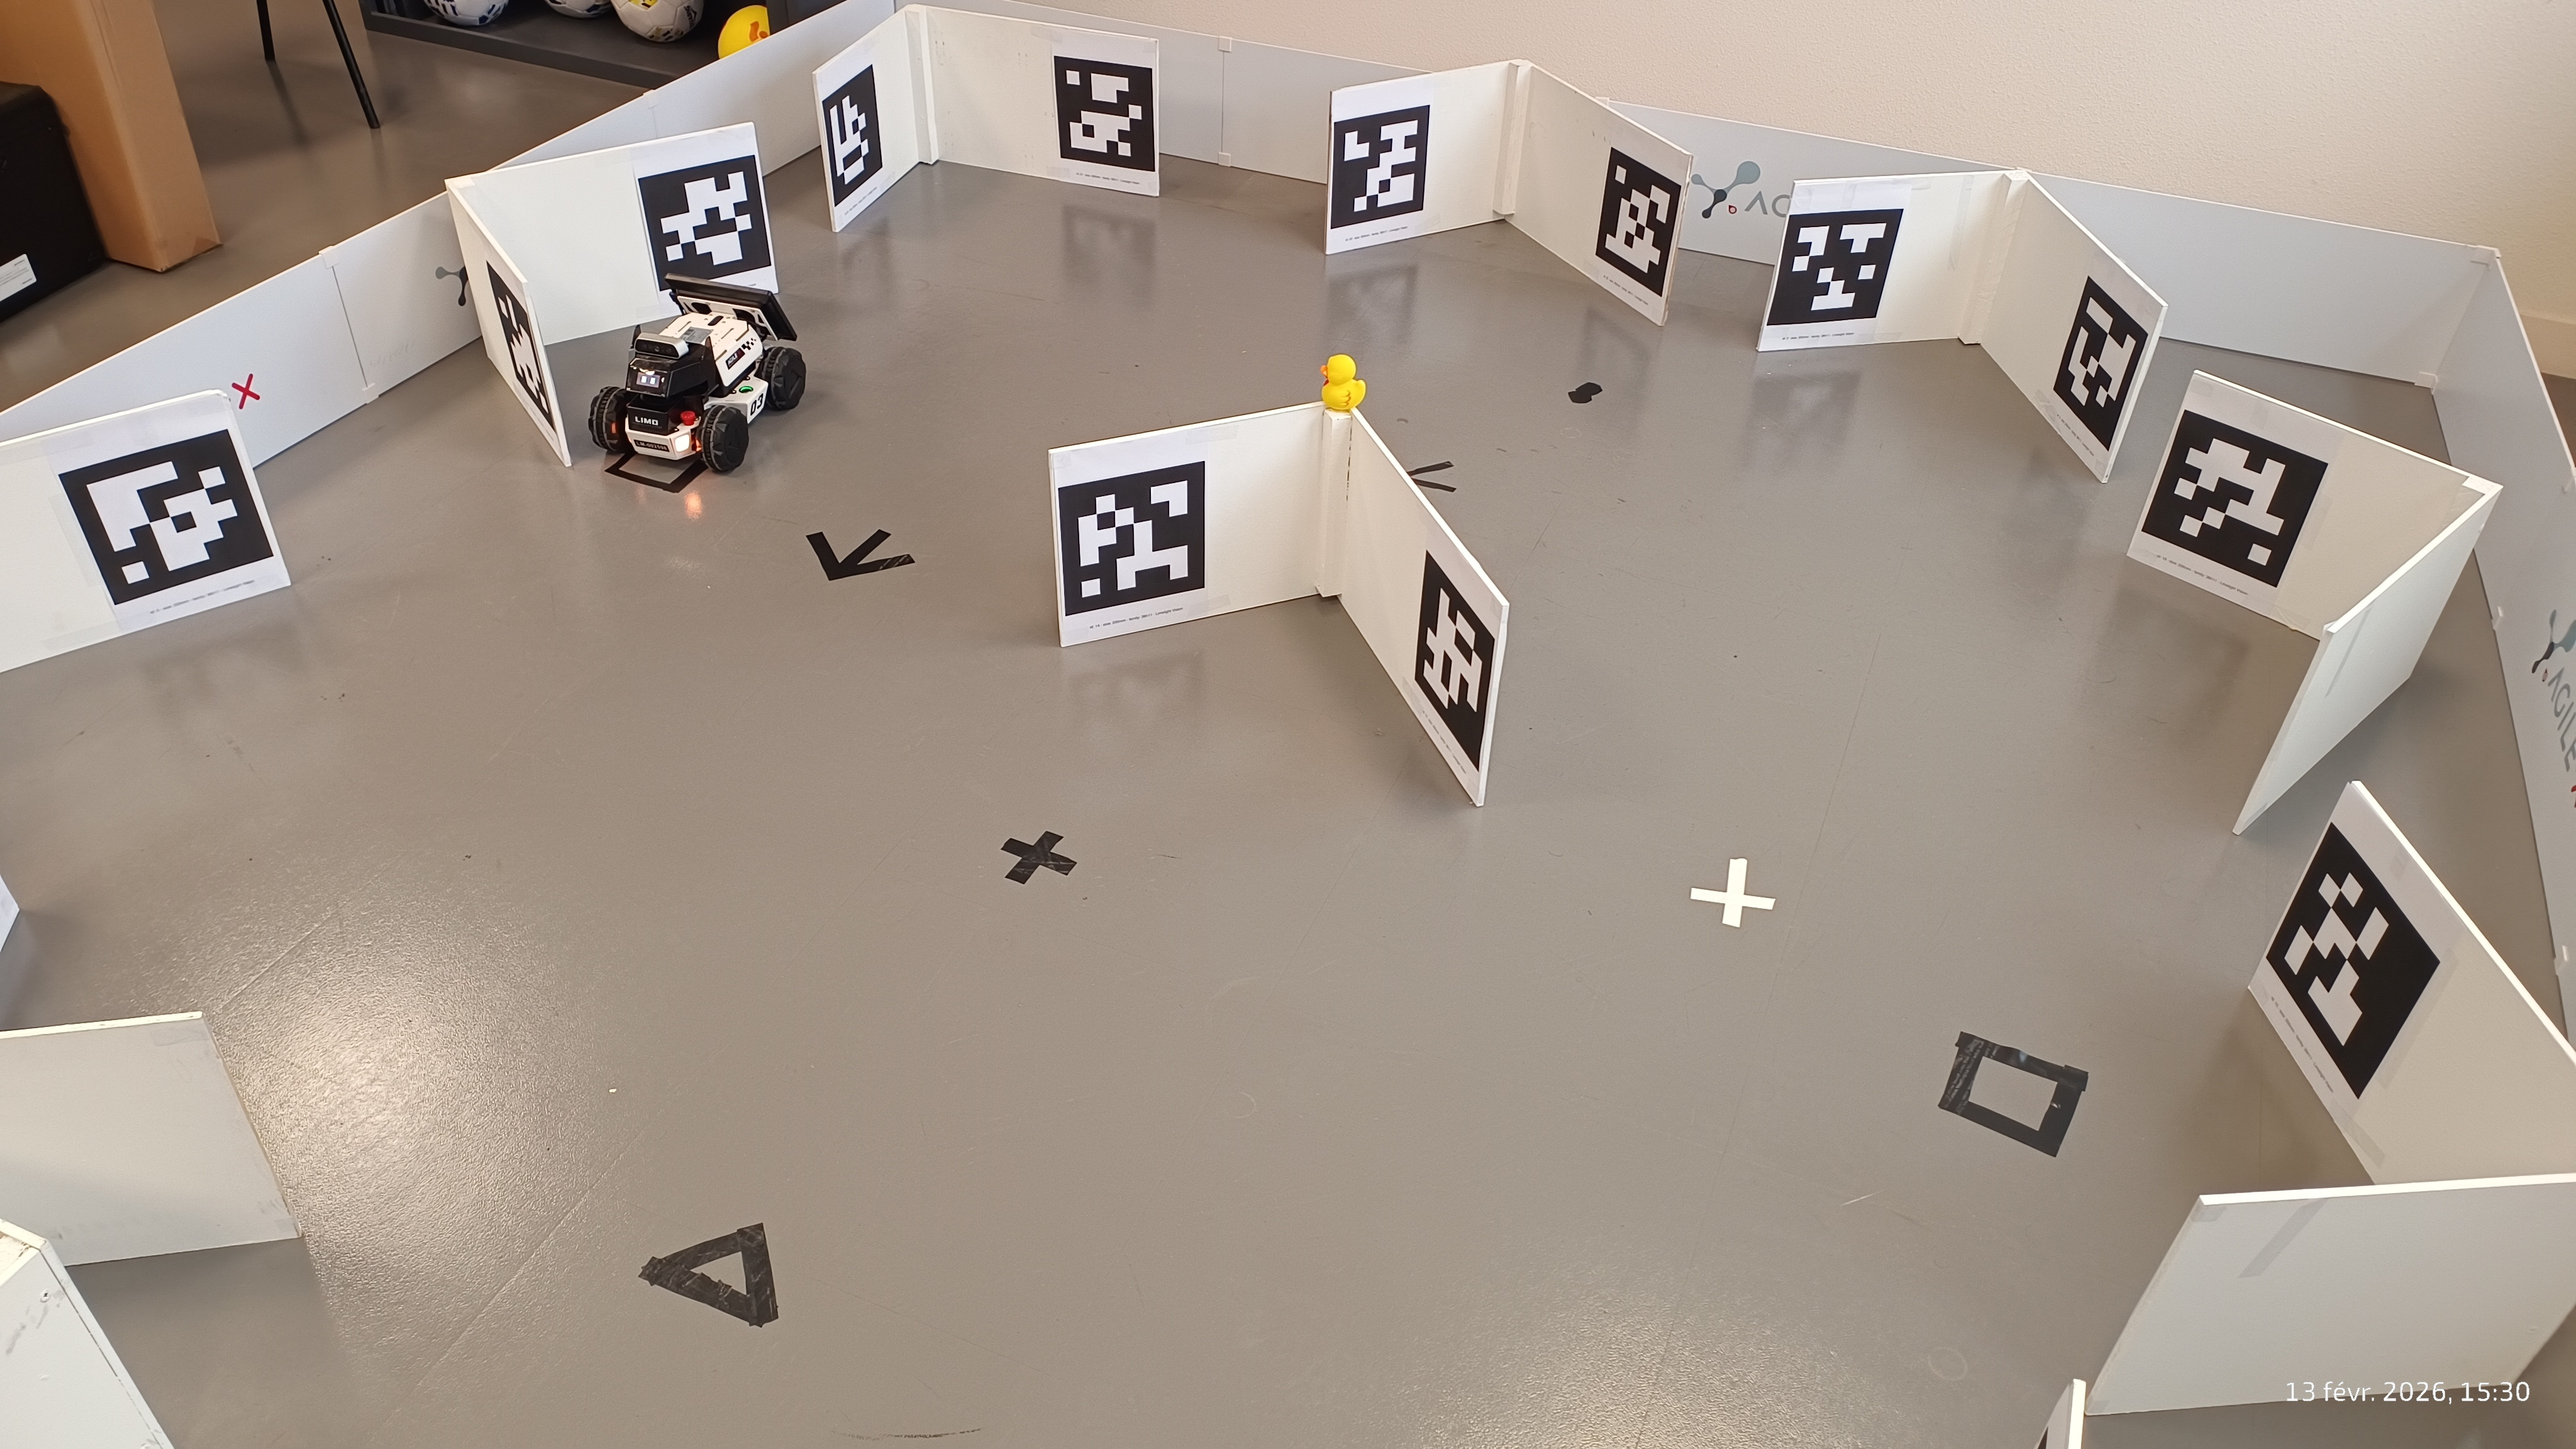
\includegraphics[width=3.35cm,height=3.30cm]{../assets/results/real_s1_reloc_13_foto.jpg}};
            \node[anchor=south west, inner sep=0pt] at (3.85,0.34)
              {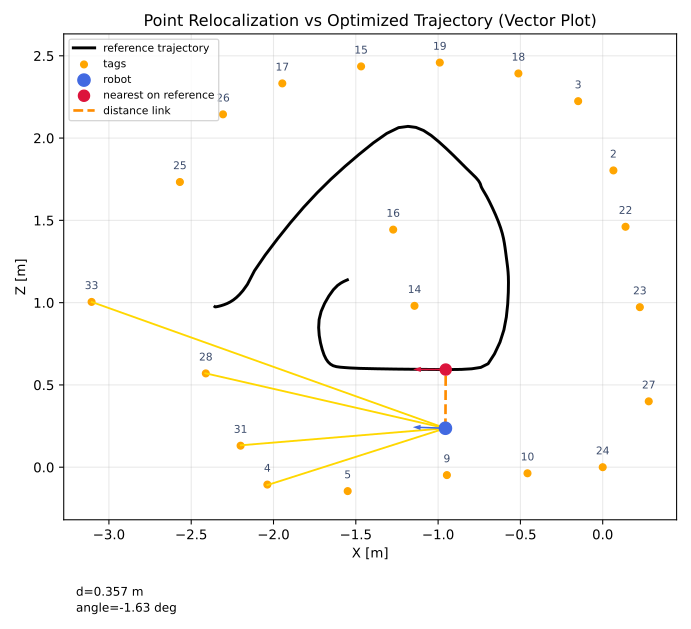
\includegraphics[width=3.35cm,height=3.30cm]{assets/results/graph_013.png}};
            \node[font=\scriptsize\bfseries, text=NavyBlue, anchor=north] at (1.98,0.30) {Point 013};
            \node[font=\scriptsize\bfseries, text=NavyBlue, anchor=north] at (5.53,0.30) {Graph 013};
          }
          % Pair 4: 015
          \only<5>{
            \node[anchor=south west, inner sep=0pt] at (0.30,0.34)
              {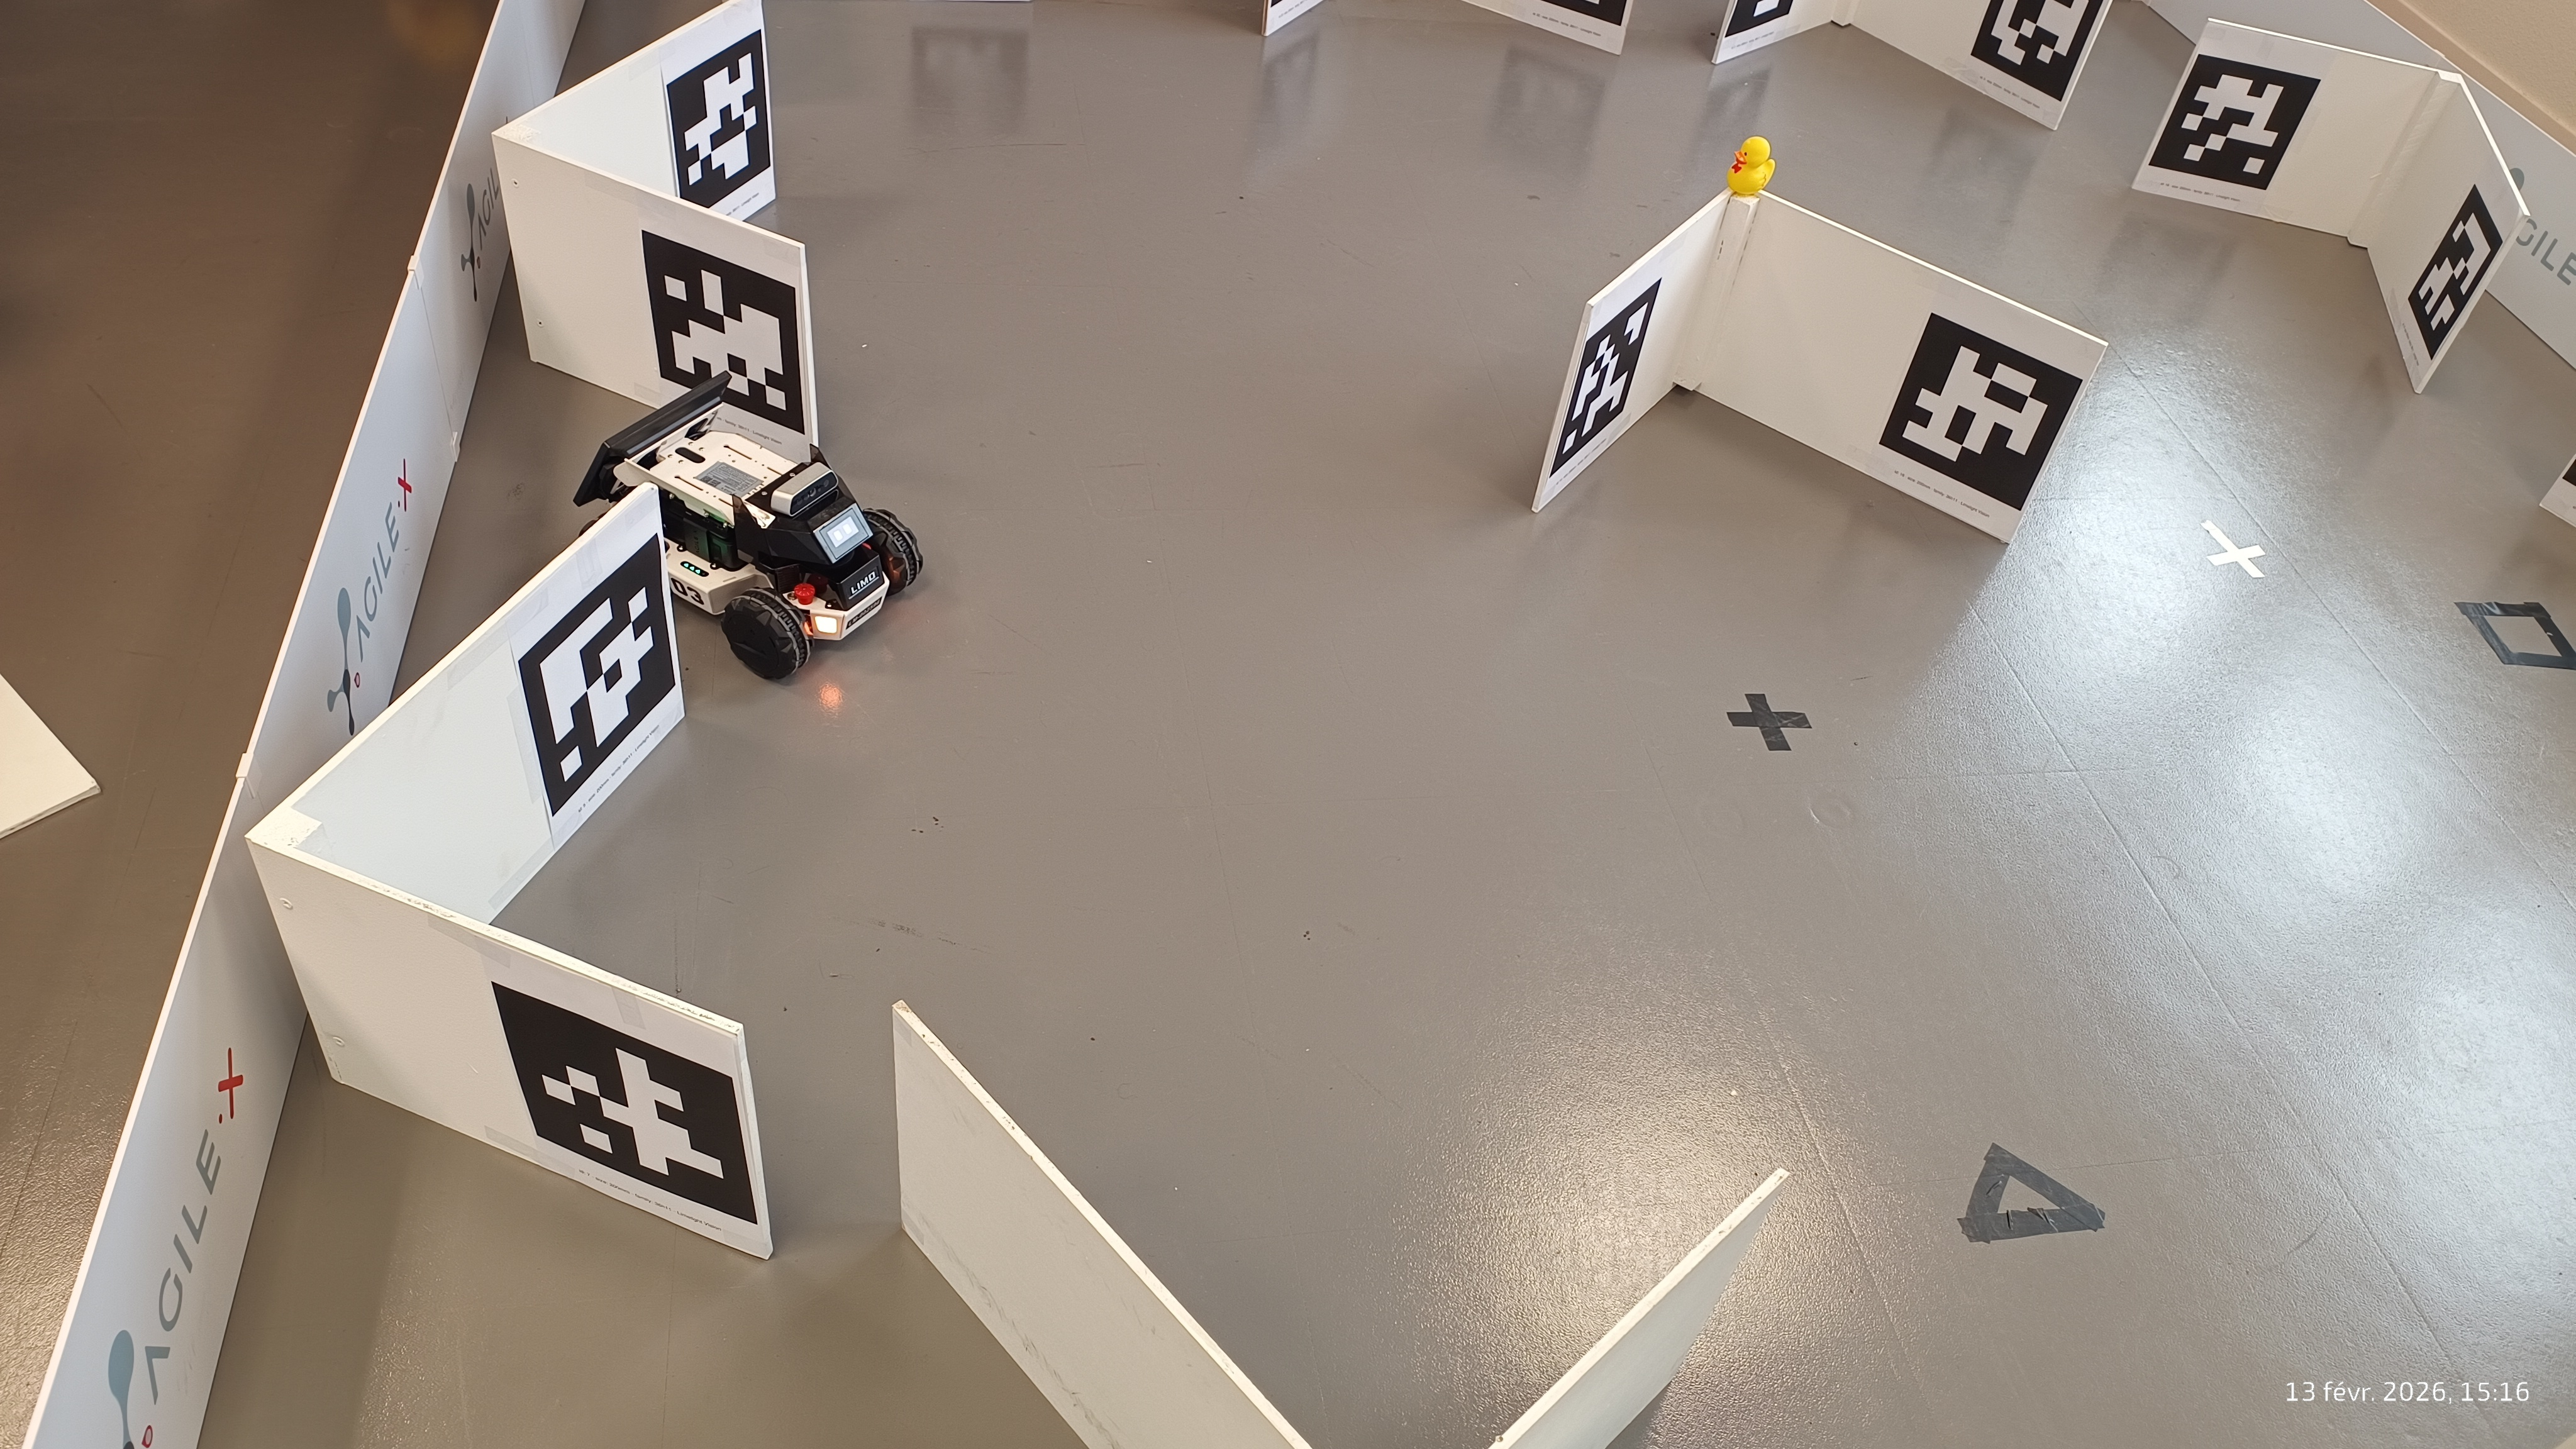
\includegraphics[width=3.35cm,height=3.30cm]{../assets/results/real_s1_reloc_015_foto.jpg}};
            \node[anchor=south west, inner sep=0pt] at (3.85,0.34)
              {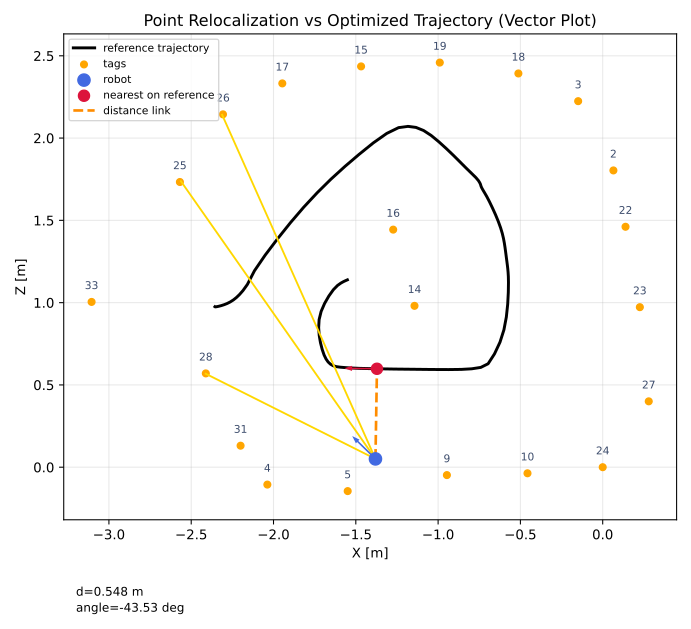
\includegraphics[width=3.35cm,height=3.30cm]{assets/results/graph_015.png}};
            \node[font=\scriptsize\bfseries, text=NavyBlue, anchor=north] at (1.98,0.30) {Point 015};
            \node[font=\scriptsize\bfseries, text=NavyBlue, anchor=north] at (5.53,0.30) {Graph 015};
          }
          % Pair 5: 016
          \only<6>{
            \node[anchor=south west, inner sep=0pt] at (0.30,0.34)
              {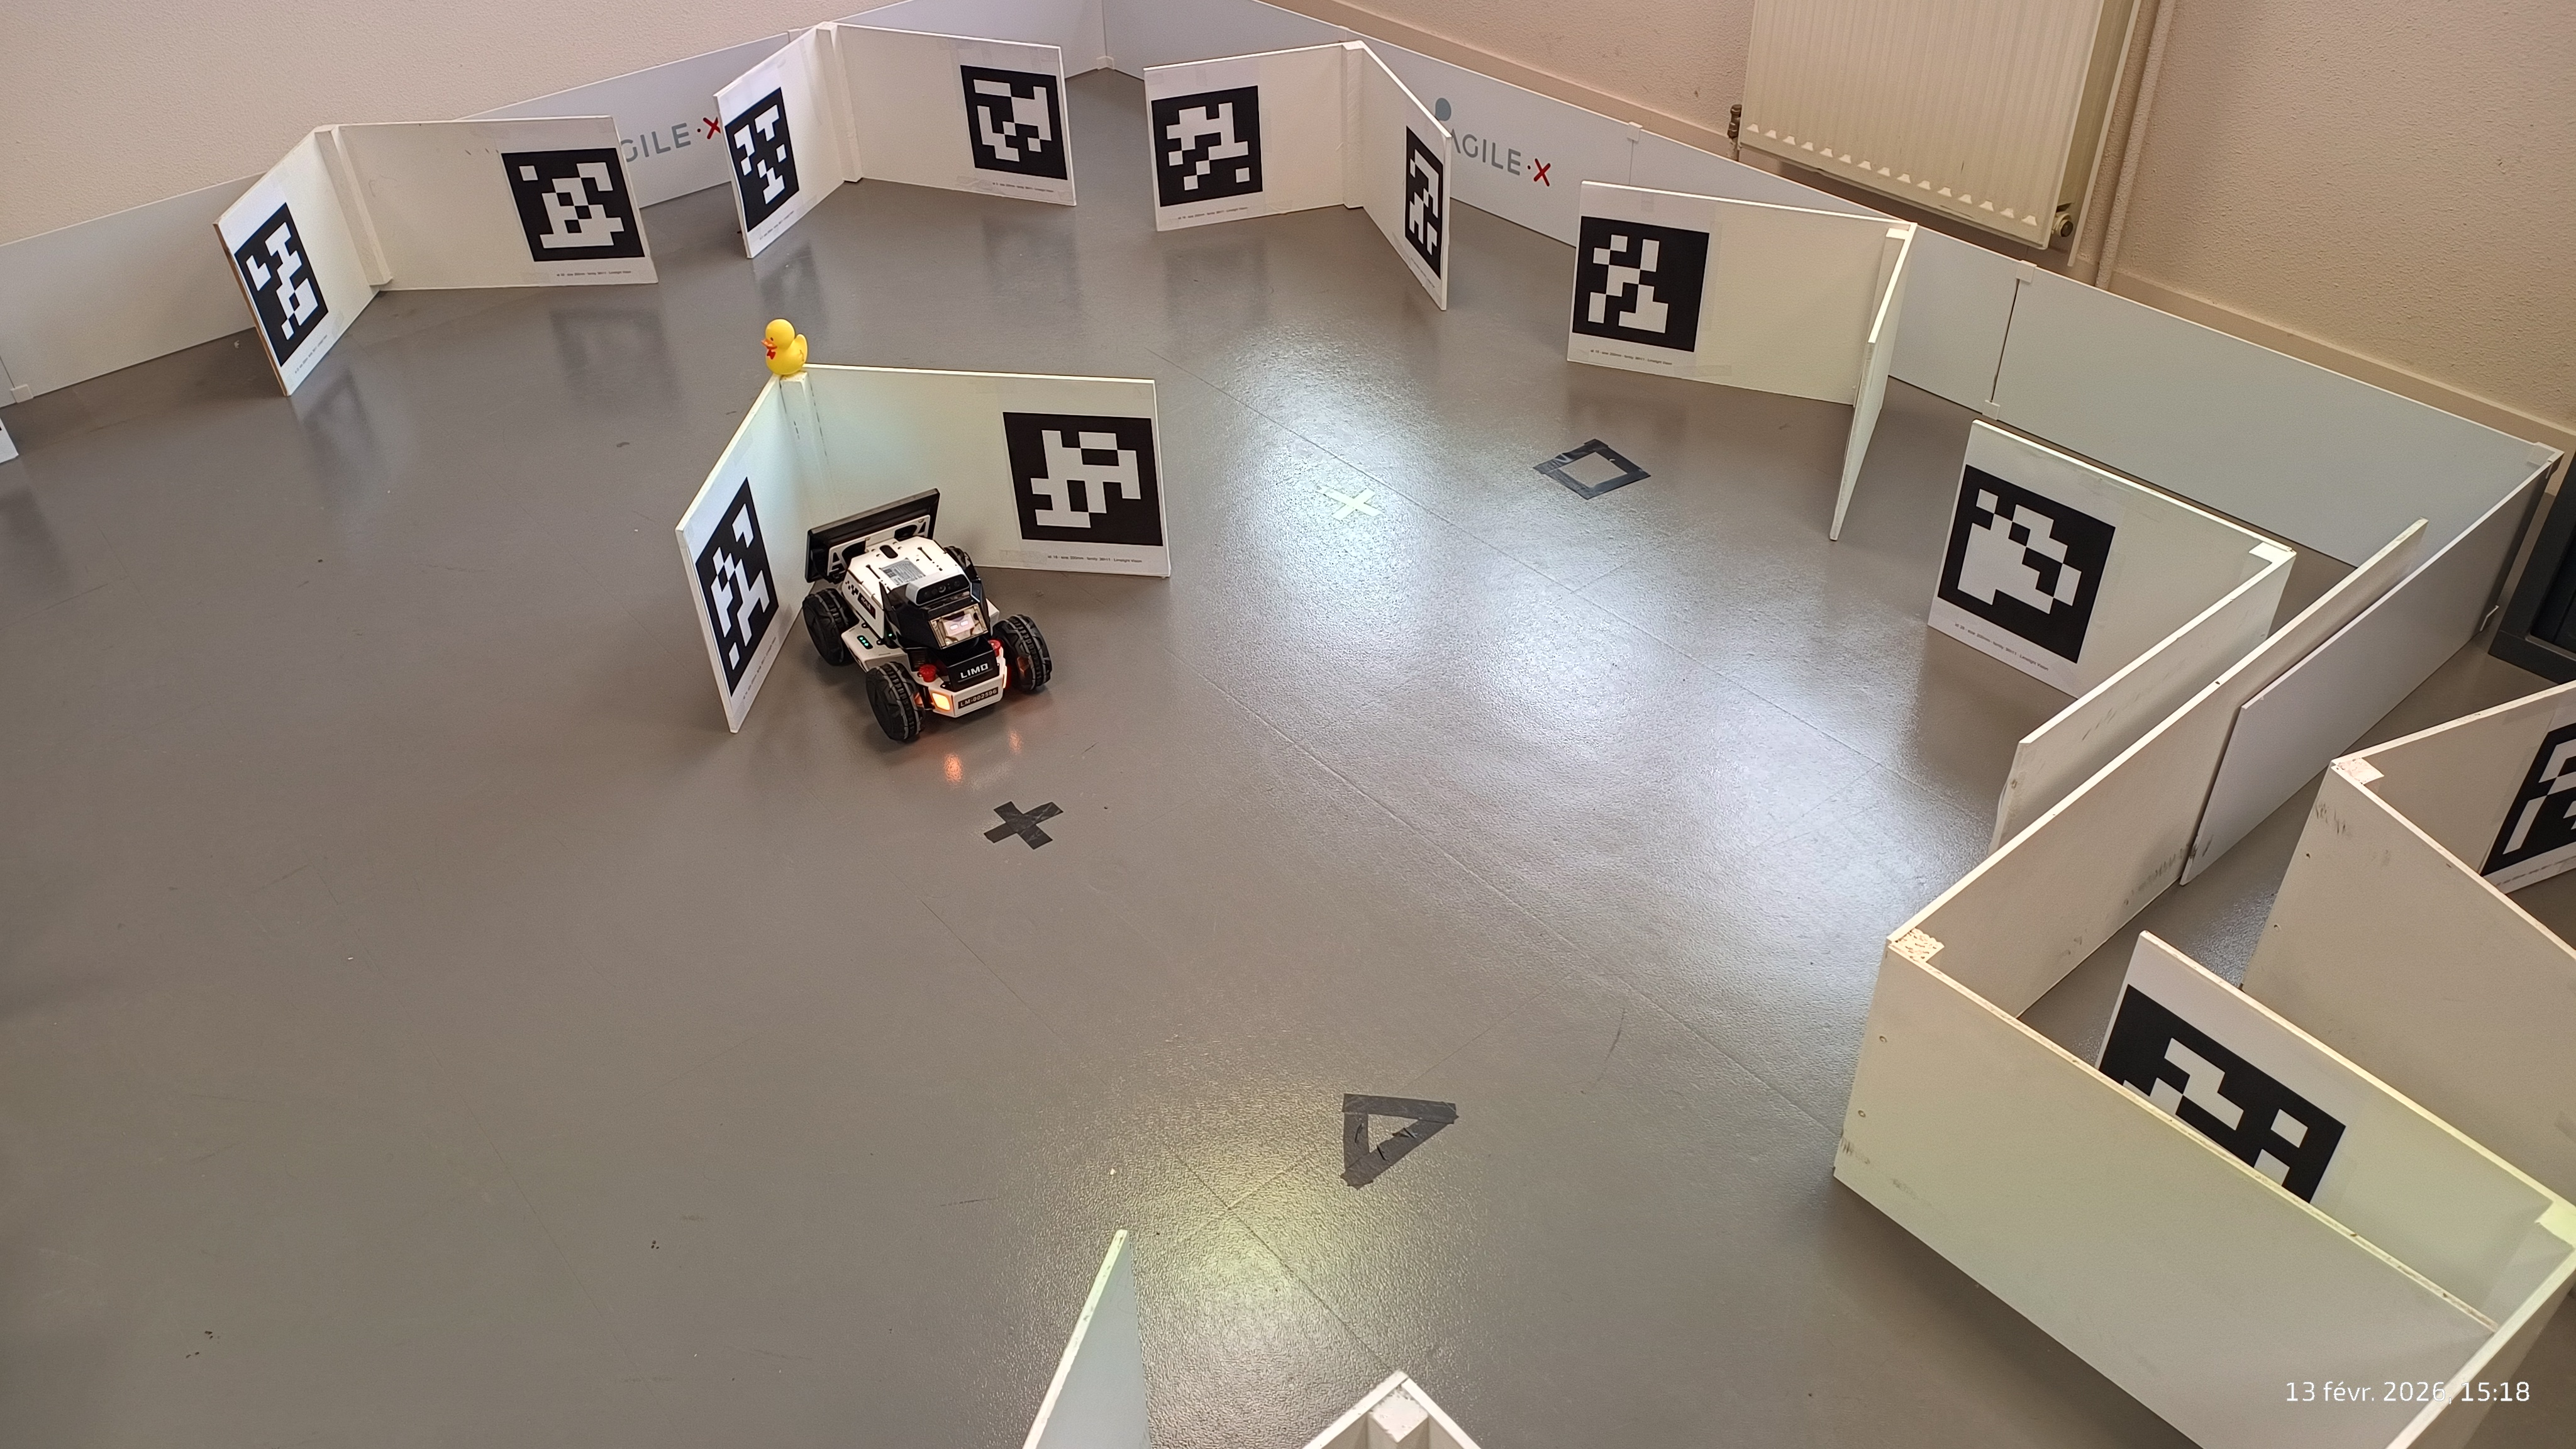
\includegraphics[width=3.35cm,height=3.30cm]{../assets/results/real_s1_reloc_016_foto.jpg}};
            \node[anchor=south west, inner sep=0pt] at (3.85,0.34)
              {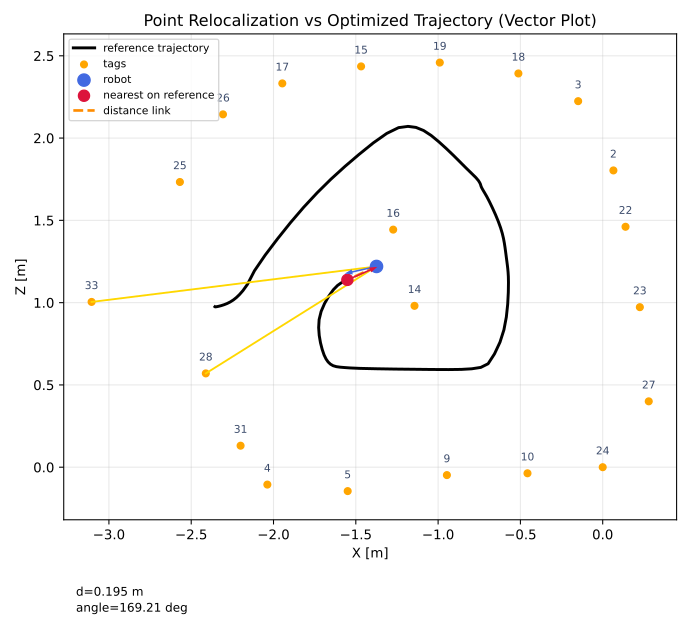
\includegraphics[width=3.35cm,height=3.30cm]{assets/results/graph_016.png}};
            \node[font=\scriptsize\bfseries, text=NavyBlue, anchor=north] at (1.98,0.30) {Point 016};
            \node[font=\scriptsize\bfseries, text=NavyBlue, anchor=north] at (5.53,0.30) {Graph 016};
          }
          % Pair 6: 018
          \only<7>{
            \node[anchor=south west, inner sep=0pt] at (0.30,0.34)
              {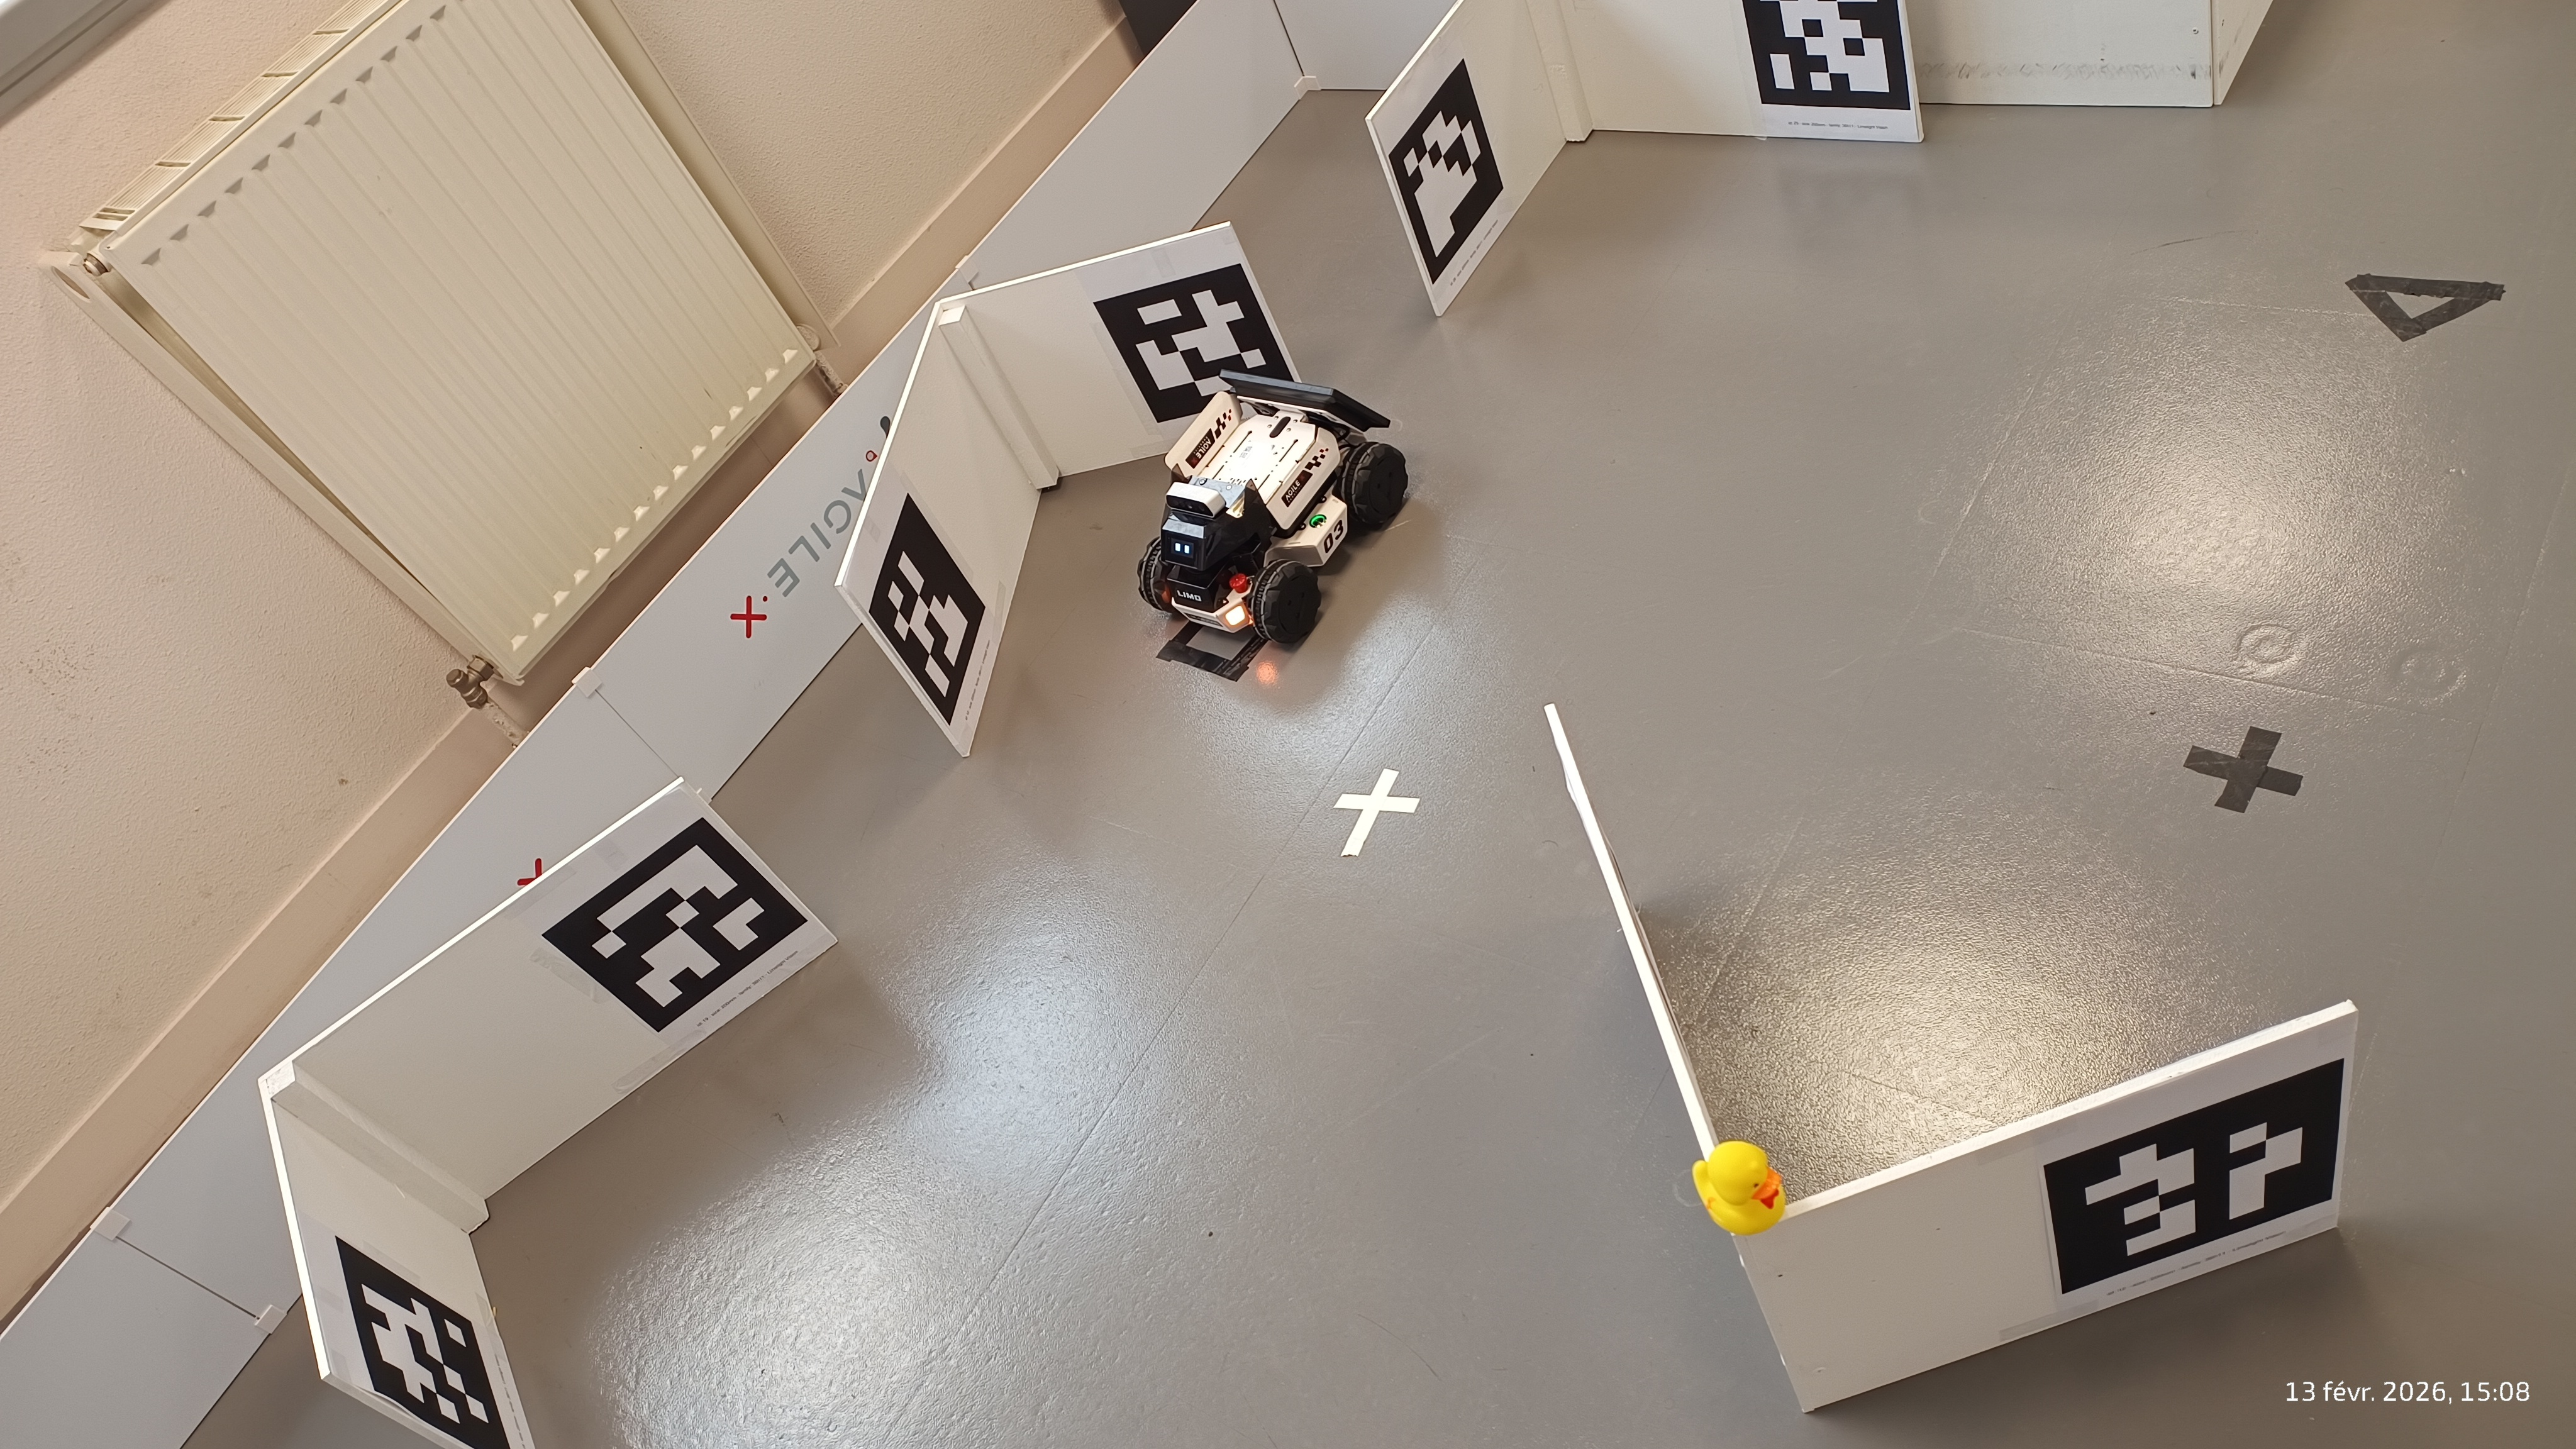
\includegraphics[width=3.35cm,height=3.30cm]{../assets/results/real_s1_reloc_018_foto.jpg}};
            \node[anchor=south west, inner sep=0pt] at (3.85,0.34)
              {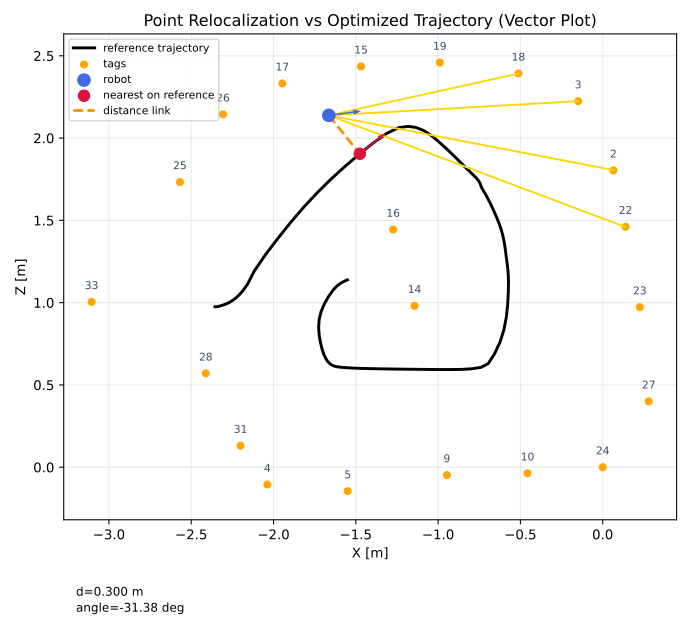
\includegraphics[width=3.35cm,height=3.30cm]{assets/results/graph_018.png}};
            \node[font=\scriptsize\bfseries, text=NavyBlue, anchor=north] at (1.98,0.30) {Point 018};
            \node[font=\scriptsize\bfseries, text=NavyBlue, anchor=north] at (5.53,0.30) {Graph 018};
          }
        \end{tikzpicture}
      }

      
    \end{outlinecard}
  \end{column}

  % ---------------- RIGHT: PIPELINE + EQUATIONS ----------------
  \begin{column}{0.35\textwidth}
    \begin{outlinecard}[Pipeline]
      \centering
      \begin{tikzpicture}[x=1cm,y=1cm,>=Latex]
        \node<1->[draw=NavyBlue!70, fill=white, rounded corners=1.2pt, line width=0.75pt,
          minimum width=3.15cm, minimum height=0.90cm, align=center] (p1) at (1.6,3.05)
          {\scriptsize\textbf{1) Previous Phase}};
        \node<2->[draw=NavyBlue!70, fill=white, rounded corners=1.2pt, line width=0.75pt,
          minimum width=3.15cm, minimum height=0.90cm, align=center] (p2) at (1.6,1.85)
          {\scriptsize\textbf{2) Match Nearest}};
        \node<3->[draw=NavyBlue!70, fill=white, rounded corners=1.2pt, line width=0.75pt,
          minimum width=3.15cm, minimum height=0.90cm, align=center] (p3) at (1.6,0.65)
          {\scriptsize\textbf{3) Metrics}};

        % active marker
        \fill<1>[AccentGold] ($(p1.north west)+(0.04,-0.04)$) rectangle ($(p1.north west)+(0.15,-0.36)$);
        \fill<2-6>[AccentGold] ($(p2.north west)+(0.04,-0.04)$) rectangle ($(p2.north west)+(0.15,-0.36)$);
        \fill<7->[AccentGold] ($(p3.north west)+(0.04,-0.04)$) rectangle ($(p3.north west)+(0.15,-0.36)$);

        % non-active marker
        \fill<2->[AccentBlue] ($(p1.north west)+(0.04,-0.04)$) rectangle ($(p1.north west)+(0.15,-0.36)$);
        \fill<7->[AccentBlue] ($(p2.north west)+(0.04,-0.04)$) rectangle ($(p2.north west)+(0.15,-0.36)$);

        \draw<2->[NavyBlue!65, line width=0.9pt, -{Latex[length=2.2mm,width=1.6mm]}] (1.6,2.58) -- (1.6,2.30);
        \draw<7->[NavyBlue!65, line width=0.9pt, -{Latex[length=2.2mm,width=1.6mm]}] (1.6,1.38) -- (1.6,1.10);
      \end{tikzpicture}
    \end{outlinecard}

    \vspace{-0.2cm}
    \only<1>{
      \begin{outlinecard}[From Previous Phase]
        \scriptsize
        
\begin{tikzpicture}[x=1cm,y=1cm]
          \node[anchor=west, text=NavyBlue, font=\scriptsize] at (0.00,0.78) {\faFile};
          \node[anchor=west, font=\scriptsize] at (0.35,0.78) {Reference trajectory};
          \node[anchor=west, font=\tiny\ttfamily] at (0.35,0.58) {trajetoria\_camera.csv};

          \node[anchor=west, text=NavyBlue, font=\scriptsize] at (0.00,0.36) {\faMapMarker};
          \node[anchor=west, font=\scriptsize] at (0.35,0.36) {Tag map};
          \node[anchor=west, font=\tiny\ttfamily] at (0.35,0.16) {tag\_map.yaml};
        \end{tikzpicture}
      \end{outlinecard}
    }

    \only<2-7>{
      \begin{outlinecard}[Nearest Projection]
        \scriptsize
        \[
          k^*=\arg\min_k \|\mathbf{p}_{\mathrm{cur}}-\mathbf{p}_k\|
        \]
        \[
          \mathbf{p}_{\mathrm{nearest}}=\mathbf{p}_{k^*}
        \]
      \end{outlinecard}
    }

    \only<7->{
      \begin{outlinecard}[Output Metrics]
        \scriptsize
        \[
          D=\|\mathbf{p}_{\mathrm{cur}}-\mathbf{p}_{\mathrm{nearest}}\|
        \]
        \[
          \phi=\mathrm{wrap}(\psi_{\mathrm{cur}}-\psi_{\mathrm{nearest}})
        \]
      \end{outlinecard}
     
    }
  \end{column}
\end{columns}
